\documentclass[11pt]{article}
\usepackage[margin=1in]{geometry} 
\usepackage{amsmath}
\usepackage{tcolorbox}
\usepackage{amssymb}
\usepackage{amsthm}
\usepackage{commath}
\usepackage{lastpage}
\usepackage{fancyhdr}
\usepackage{accents}
\usepackage{csquotes}
\usepackage{soul}
\newcommand{\ubar}[1]{\underaccent{\bar}{#1}}
\pagestyle{fancy}
\setlength{\headheight}{40pt}


\newenvironment{solution}
  {\renewcommand\qedsymbol{$\blacksquare$}
  \begin{proof}[Solution]}
  {\end{proof}}
\renewcommand\qedsymbol{$\blacksquare$} 
\begin{document}

\lhead{Yida Liu} 
\rhead{EECS 416 Spring 2020 \\ Convex Optimization for Engineering \\ Homework 2} 
\cfoot{\thepage\ of \pageref{LastPage}}

\section{Solve Sunco Oil Problem with \texttt{linprog}}

\begin{figure}[h]
    \centering
    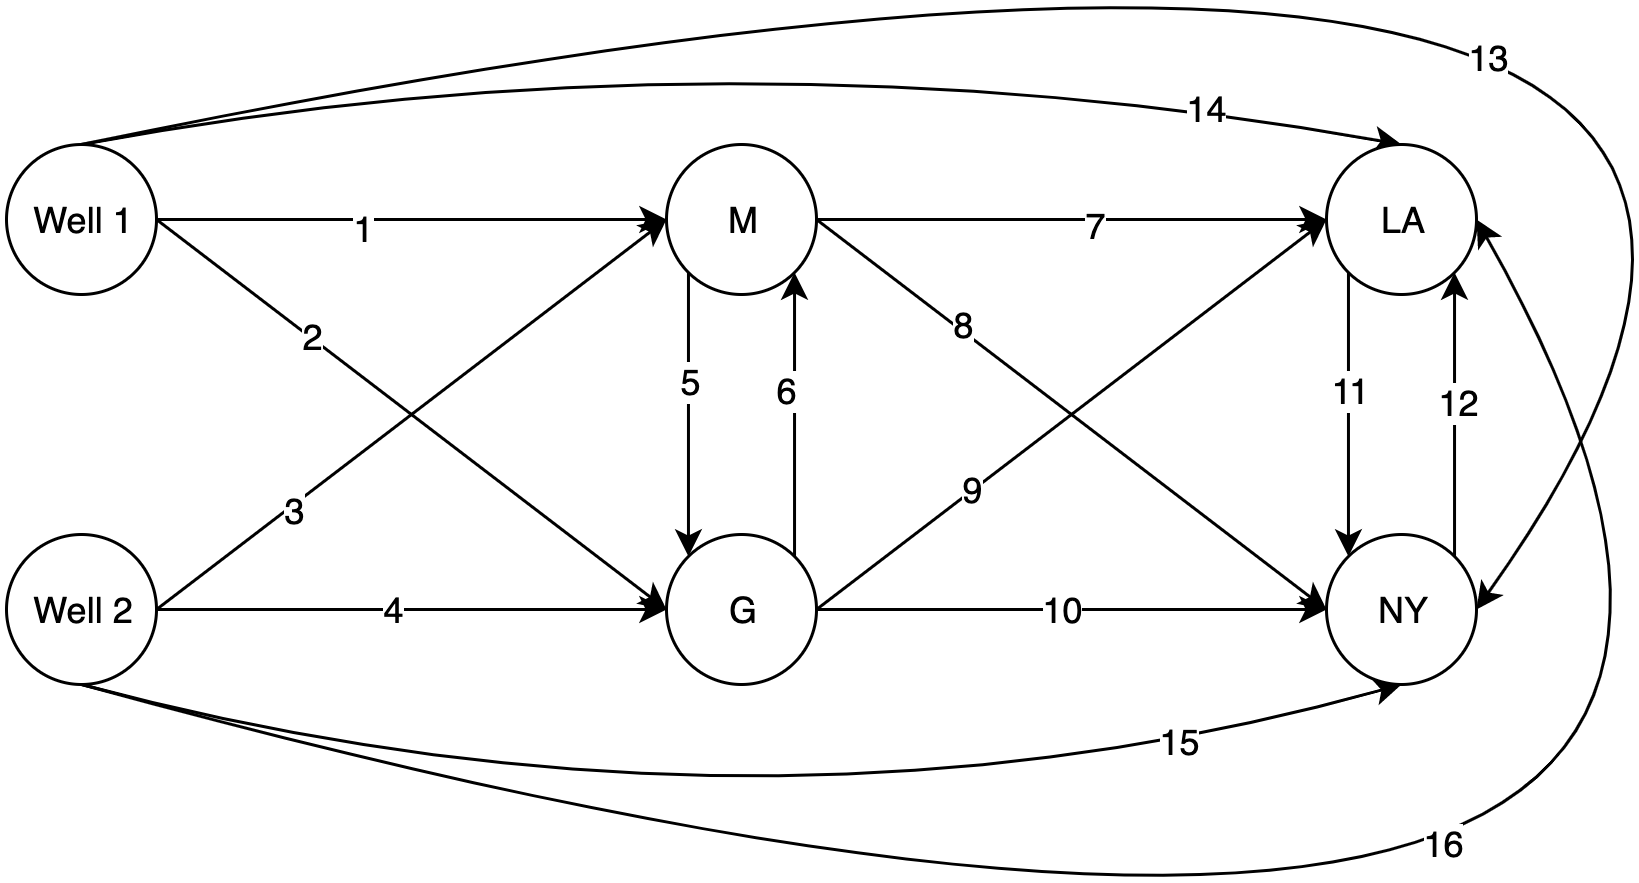
\includegraphics[width=0.9\linewidth]{hw1/hw1-prob2-graph.png}
    \caption{Network Flow of Sunco Oil Problem}
\end{figure}

Let us have the complete model first:
\begin{align*}
&\min && \sum_i C_ix_i \\
&s.t.
 && x_1 + x_3 + x_6 - x_5 - x_7 - x_8 = 0&(\text{Mobile cleared})\\
&&&x_2 + x_4 + x_5 - x_6 - x_9 - x_{10} =  0&(\text{Galveston cleared}) \\
&&& x_7 + x_9 - x_{11} + x_{12} + x_{14} + x_{16} \geq 170 &(\text{LA demand})\\
&&& x_8 + x_{10} + x_{11} - x_{12} + x_{13} + x_{15} \geq 150 &(\text{NY demand}) \\
&&&x_1 + x_2 + x_{13} + x_{14} \leq 180 &(\text{Well 1 supply})\\
&&& x_3 + x_4 + x_{15} + x_{16} \leq 210 &(\text{Well 2 supply}) \\
&&& \forall i \in [1,...,16], x_i \geq 0 & (\text{Non-negativity})
\end{align*}

\textbf{Solution}\par
The solution from MATLAB \texttt{linprog} advises that we ship 110, 210, 110, 60, 150 on edge 1, 4, 7, 9, and 10, respectively. That is to say: 
\begin{enumerate}
    \item Well 1 ships 110,000 bbl to Mobile
    \item Well 2 ships 210,000 bbl to Galveston
    \item Mobile ships all 110,000 bbl to LA
    \item Galveston ships 60,000 bbl to LA and 150,000 bbl to NY.
\end{enumerate}
The optimal objective value is 8090. Note that although the optimal objective value is the same with the previous solution we had in Homework 1 with Excel Solver, the two solution actually differs. It is probable for this linear programming problem to have multiple optimial solutions. 

\section{Solve Manufacturing Process with \texttt{linprog}}

\textit{The precision of the displayed numbers are limited to 4 decimal places.}

Again, let us have the complete model first:

\begin{align*}
&\max && 4.71269x_1 + 3.86654x_2 + 3.48825x_3 & (\text{Maximize total profit})\\
&s.t
 && 0.5814x_1 + 0.54506x_2 \leq 1700 & (\text{Max daily sales A}) \\
&&& 0.612x_3 \leq 1500 & (\text{Max daily sales B}) \\
&&& 0.5814x_1 + 0.54506x_2 + 0.612x_3 \leq 2500 & (\text{Shipping limit}) \\
&&& 0.0033x_1 + 0.0033x_2 + 0.002x_3 \leq 16 & (\text{Facility 1 hours}) \\
&&& 0.0038x_1 + 0.002x_2 \leq 12 & (\text{Facility 2 hours}) \\
&&& 0.0021x_2 + 0.0019x_3 \leq 12 & (\text{Facility 3 hours}) \\
&&& 0.0034x_1 + 0.0034x_2 + 0.0019x_3 \leq 16 & (\text{Facility 4 hours}) \\
&&& \forall i \in [1,2,3], x_i \geq 0 & (\text{Non-negativity}) \\
\end{align*}

\textbf{Solution:}\par
The solution from MATLAB \texttt{linprog} suggests using 2923.9766 and 1307.1895 gallons of raw materials on process 1 and 2, which would eventually yield a profit of \$18340 (or \$18339.5919, to be specific). This solution results in final production of 1700 and 800 gallons of product A and B. This solution is consistent with the previous solution in Homework 1 with Excel Solver.

\section{Circle from Rubber}

\textbf{Decision variables}\par
The center of the circle $C_i=(x_i, y_i)$, and the radius $r_i$, for $i \in [1, 2, 3]$

\textbf{Objective function}\par
The problem seeks to minimize the waste after cutting, which is equivalent to say the total shape of the circles are maximized. 
$$
\max \pi\sum_i r_i^2
$$

\textbf{Constraints}
\begin{enumerate}
    \item Non-overlapping circles: circles cannot overlap, otherwise it would not be the shape of the circle when cut. The distance between the center of two circle must be larger than the sum of their radii. Therefore, for each combination of circle $i$ and $j$, we must have constraint
    $$
    (x_i - x_j)^2 + (y_i - y_j)^2 \geq (r_i + r_j)^2
    $$
    
    \item Circle within bound: circles must be enclosed by the polygon that the points formed. To formulate this, we consider that the distance from the circle center to each of the edges of the polygon must be greater than the radius of the circle. We know how to calculate the formula for lines given two points m and n:
    $$
    ax + by = c, a = (x_m - x_n), b = (x_n - x_m), c = x_my_n - x_my_n
    $$
    Then we consider that for a circle i within the polygon bound, we have $ax_i + by_i \leq c$, then the distance from point i to the line,
    $$
    d = \frac{c - ax_i - by_i}{\sqrt{a^2 + b^2}}
    $$
    We must have $d \geq r_i$.
    
    \item Non-negativity: radius must be greater than zero.
\end{enumerate}

\textbf{Model:}
\begin{align*}
&\min&& -\pi \sum_{i=1}^3 r_i^2 \\
&s.t.
 && (x_1 - x_2)^2 + (y_1 - y_2)^2 \geq (r_1 + r_2)^2 &(\text{Circle 1 and 2 not overlap})\\
&&& (x_1 - x_3)^2 + (y_1 - y_3)^2 \geq (r_1 + r_3)^2 &(\text{Circle 1 and 3 not overlap})\\
&&& (x_2 - x_3)^2 + (y_2 - y_3)^2 \geq (r_2 + r_3)^2 &(\text{Circle 2 and 3 not overlap}) \\
&&& \forall i \in [1,2,3], r_i - y_i \leq 0 &(\text{Circle within bound 1}) \\
&&& \forall i \in [1,2,3], \sqrt{37}r_i - 6x_i + y_i \leq 0 & (\text{Circle within bound 2}) \\
&&& \forall i \in [1,2,3], \sqrt{53}r_i + 2x_i + 7y_i \leq 440 & (\text{Circle within bound 3}) \\
&&& \forall i \in [1,2,3], \sqrt{13}r_i + 3x_i + 2y_i \leq 235 & (\text{Circle within bound 4}) \\
&&& \forall i \in [1,2,3], \sqrt{17}r_i + 4x_i + y_i \leq 200 & (\text{Circle within bound 5}) \\
\end{align*}

\textbf{Solutions}\par

\begin{figure}
    \centering
    \begin{tabular}{c  c}
        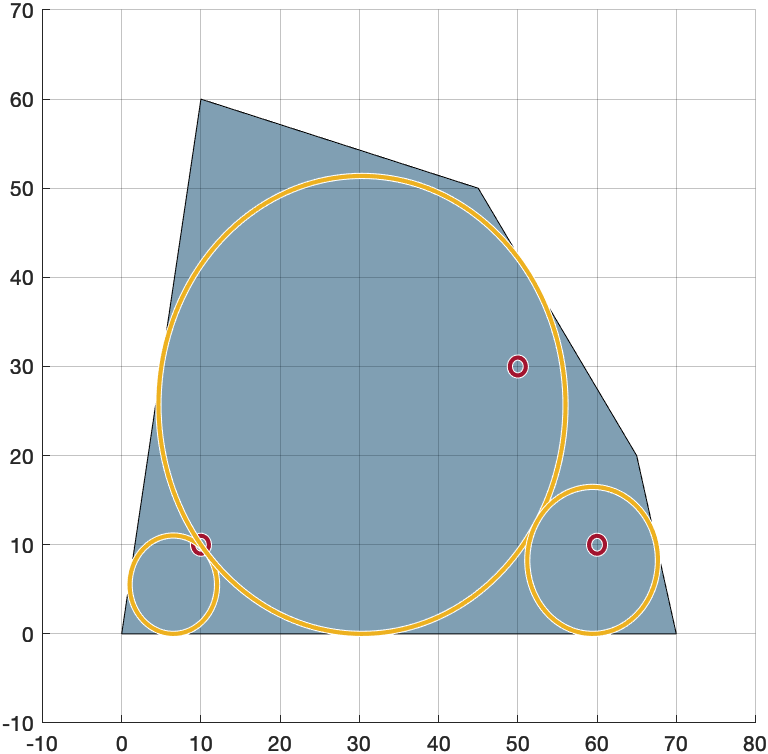
\includegraphics[width=0.4\linewidth]{hw2/hw2-prob1-plot1.png} &
        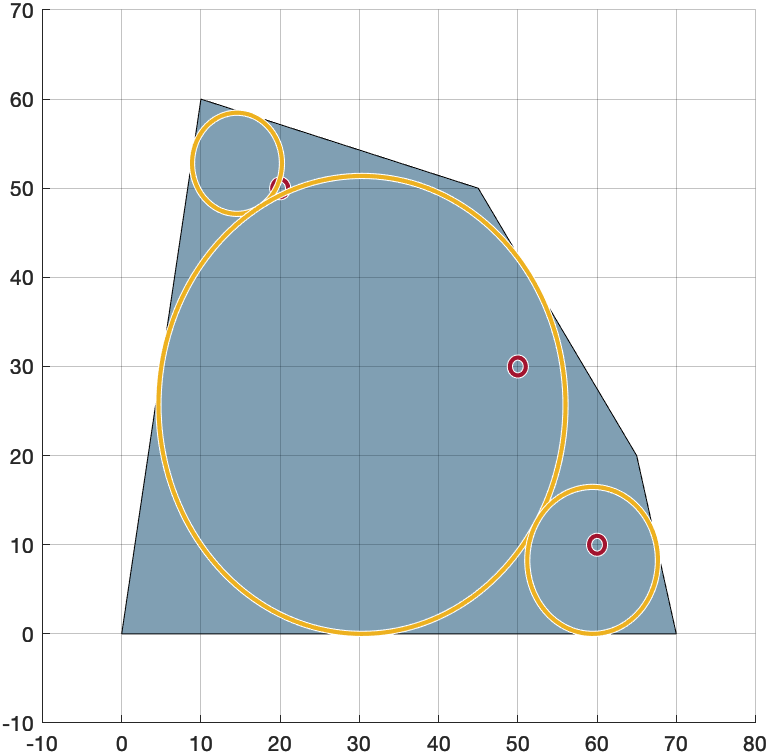
\includegraphics[width=0.4\linewidth]{hw2/hw2-prob1-plot2.png}
    \end{tabular}
    \caption{A Local Minimum (left) and A Better One (right)}
    \label{fig:circle_better_minima_cmp}
\end{figure}

We use MATLAB \texttt{fmincon} to solve this problem. The below table shows the first solution with object value -2382.93646.
\begin{center}
\begin{tabular}{c || c | c | c || c | c | c}
     circle & r0 & x0 & y0 & r & x & y \\
     \hline
     1     & 1  & 10 & 10 & 5.5183 & 6.5142 & 5.5183 \\
     2     & 1  & 50 & 30 & 25.6917 & 30.328 & 25.6917 \\
     3     & 1  & 60 & 10 & 8.24611 & 59.4386 & 8.24611 \\
\end{tabular}
\end{center}

We display the solution as a plot as shown in Figure \ref{fig:circle_better_minima_cmp}. The red circle (tiny) are the initial solution and the yellow circle (large) are the optimal solution.

After inspecting the left plot, we there might be a better solution, as it is obvious there are seemingly more space on the upper-left corner. Therefore we changed the initial starting point and re-run the program and we achieved a better object value of -2388.37652. The result is shown in the table below. 

\begin{center}
\begin{tabular}{c || c | c | c || c | c | c}
     circle & r0 & x0 & y0 & r & x & y \\
     \hline
     1     & 1  & 20 & 50 & 5.67305 & 14.5512 & 52.7669 \\
     2     & 1  & 50 & 30 & 25.6917 & 30.328 & 25.6917 \\
     3     & 1  & 60 & 10 & 8.24611 & 59.4386 & 8.24611 \\
\end{tabular}
\end{center}

\section{Power Generator Placement}

\begin{figure}[h]
    \centering
    \begin{minipage}{.46\textwidth}
        \centering
        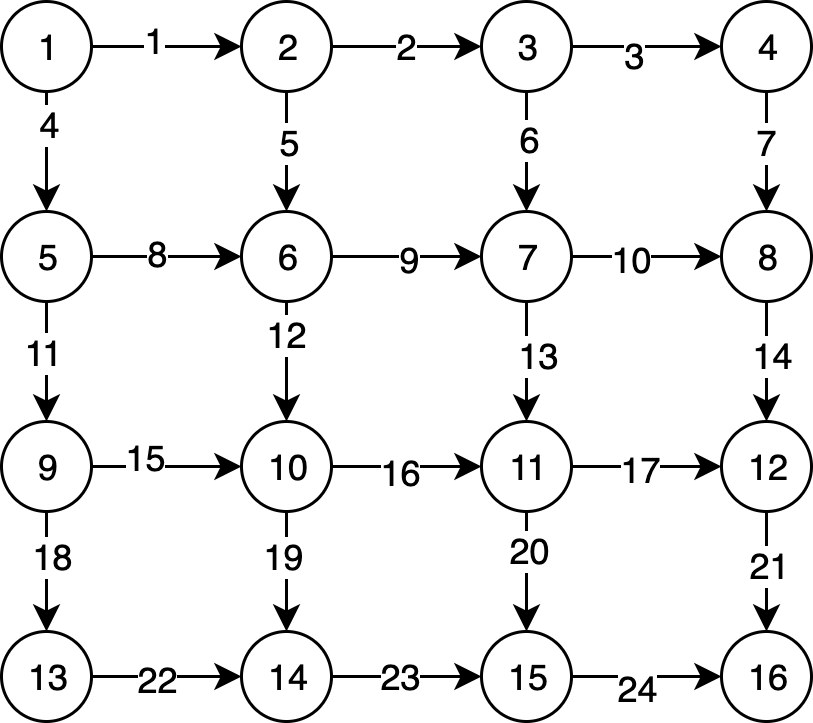
\includegraphics[width=0.9\linewidth]{hw2/hw2-prob4.png}
        \caption{A Directed Graph of the Nodes and Possible Location of Power Lines (labeled)}
        \label{fig:dag_power}
    \end{minipage}%
    \begin{minipage}{.46\textwidth}
        \centering
        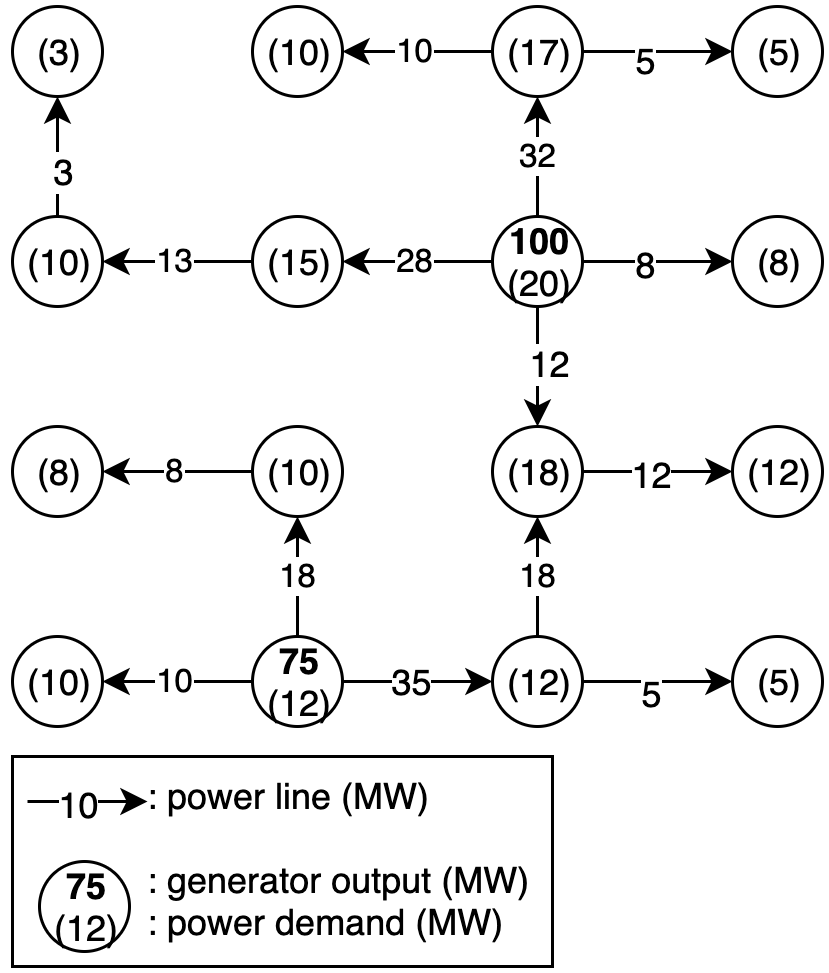
\includegraphics[width=0.8\linewidth]{hw2/hw2-prob4-sol.png}
        \caption{Solution for Power Generator Placement (with reversed negative edges)}
        \label{fig:sol_power}
    \end{minipage}
\end{figure}


\textbf{Definitions}\par
\begin{enumerate}
\item $i$ the identifier of node, $i \in [1,...,16]$
\item $j$ the identifier of arc, $j \in [1,...,24]$
\item $y_i$ generator presence at node $i$ (binary)
\item $s_i$ the size of generator at node $i$ (MW)
\item $d_i$ the demand of energy at node $i$ (MW)
\item $e_i$ the available energy at node $i$ (MW)
\item $l_j$ the energy transmitted in arc $j$ with direction regard to arc location (MW)
\item $p_j$ the energy transmitted in arc $j$ regardless of direction (MW); that is $p_j = \abs{l_j}$
\end{enumerate}

\textbf{Decision Variables:} $y_i$, $s_i$, $e_i$, $l_j$, $p_j$

\textbf{Objective Function}\par
\begin{align*}
&\min && \sum_i (100 y_i + 2s_i) + \sum_j 1.5p_j && (Total Cost)\\
\end{align*}

\textbf{Constraints}
\begin{enumerate}
\item Generator Presence\par
If no generator presence, the output would be zero. In addition, the maximum size is 100MW. 
\begin{align*}
&&& - 100y_i + s_i \leq 0 & i \in [1,...,16] & (\text{Generator presence})\\
\end{align*}

\item Power Output Limit\par
The power output at node cannot exceed the size.
\begin{align*}
&&& - s_i + e_i \leq 0 & i \in [1,...,16] & (\text{Power output limit})\\
\end{align*}

\item Absolute Power Transmission\par
Absolute value is not linear, as we have $p_j = \abs{l_j}$, we can convert to
\begin{align*}
&&& l_j - p_j \leq 0 & j \in [1,...,24] & (\text{Absolute Power Transmission High}) \\
&&& -l_j - p_j \leq 0 & j \in [1,...,24] & (\text{Absolute Power Transmission Low}) \\
\end{align*}

\item Generator in Tile\par
Environmental restrictions says that no two generator may be less than 1.5 miles apart. It is essentially saying that each tile on the graph has at most 1 generator.
\begin{align*}
&&& y_1 + y_2 + y_5 + y_6 \leq 1 && (\text{Generator in Tile 1}) \\
&&& y_2 + y_3 + y_6 + y_7 \leq 1 && (\text{Generator in Tile 2}) \\
&&& y_3 + y_4 + y_7 + y_8 \leq 1 && (\text{Generator in Tile 3}) \\
&&& y_5 + y_6 + y_9 + y_{10} \leq 1 && (\text{Generator in Tile 4}) \\
&&& y_6 + y_7 + y_{10} + y_{11} \leq 1 && (\text{Generator in Tile 5}) \\
&&& y_7 + y_8 + y_{11} + y_{12} \leq 1 && (\text{Generator in Tile 6}) \\
&&& y_9 + y_{10} + y_{13} + y_{14} \leq 1 && (\text{Generator in Tile 7}) \\
&&& y_{10} + y_{11} + y_{14} + y_{15} \leq 1 && (\text{Generator in Tile 8}) \\
&&& y_{11} + y_{12} + y_{15} + y_{16} \leq 1 && (\text{Generator in Tile 9}) \\
\end{align*}

\item Generator in Coordinate Line \par
Environmental restrictions specifies that no more than two generators may be built on any coordinate line.
\begin{align*}
&&& y_1 + y_2 + y_3 + y_4 \leq 2 && (\text{Generator in x-coordinate 1}) \\
&&& y_5 + y_6 + y_7 + y_8 \leq 2 && (\text{Generator in x-coordinate 2}) \\
&&& y_9 + y_{10} + y_{11} + y_{12} \leq 2 && (\text{Generator in x-coordinate 3}) \\
&&& y_{13} + y_{14} + y_{15} + y_{16} \leq 2 && (\text{Generator in x-coordinate 4}) \\
% y-coord
&&& y_1 + y_5 + y_9 + y_{13} \leq 2 && (\text{Generator in y-coordinate 1}) \\
&&& y_2 + y_6 + y_{10} + y_{14} \leq 2 && (\text{Generator in y-coordinate 2}) \\
&&& y_3 + y_{7} + y_{11} + y_{15} \leq 2 && (\text{Generator in y-coordinate 3}) \\
&&& y_{4} + y_{8} + y_{12} + y_{16} \leq 2 && (\text{Generator in y-coordinate 4}) \\
\end{align*}

\item Generator Pair \par
Environmental restriction specifies that if a generator is built at node 4, then another must be build on node 13. 
\begin{align*}
&&& y_4- y_{13} \leq 0 & &(\text{Generator Pair 4 - 13})
\end{align*}

\item Power Equilibrium \par
The power input enters a node equals the output the node. 
As shown in the hint:
\begin{align*}
&&& e_i + B_i l = d_i & i \in [1,...,16] & (\text{Power Equilibrium}) \\
\end{align*}
, where $B$ is the incidence matrix constructed from the graph. 


\item Model Variable Integrity \par
There are several integrity rules to follow: including non-negativity and integer constraints
\begin{align*}
&&& y_i \in \mathbb{Z} \land y_i \in [0, 1] & i \in [1,...,16] & (\text{Integer}) \\
&&& s_i, e_i \geq 0 & i \in [1,...,16] & (\text{Non-negativity 1}) \\
&&& p_j \geq 0 & j \in [1,...,24] & (\text{Non-negativty 2}) \\
&&& l_j \text{ unconstrained} &  j \in [1,...,24] & \\
\end{align*}
\end{enumerate}
This summarizes the model we built for solving this problem.


\textbf{Solution:}\par

Here we present the solution that came out from MATLAB \texttt{intlinprog}. The solution gives an cost of \$875.5. The solution suggests that we build a 100-MW generator at node 7 and a 75-MW generator at node 14, with a number of power lines being built to connect all nodes and satisfy all power demand. The solution is presented in Figure \ref{fig:sol_power}, where all the negative power line transmission are adjusted to forward edges. 

In addition, it is worthwhile noting that there exist more than one solution for this problem. When the placements of power generators are determined, it is trivial to place all the connecting power lines.

\end{document}